\chapter{Multi-bit Spike Train Model}
\label{chap:multi-bit-spike-train-model}

\section{Graded Spikes}
\label{sec:graded-spikes}
    Now we consider the firing model with graded spikes, namely our multi-bit spike train model. We divide the range of $[0, \theta]$ into
    $2^n-1$ intervals where $n$ is the number of bits used to encode one single spike. Then once the membrane potential reaches the threshold 
    for a certain interval, the neuron fires a spike with the corresponding intensity described as follows:
    \begin{equation}
        S_{\text{out}}[t] = \begin{cases}
            0               & \text{if } U[t] < \frac{1}{2^n-1}\cdot\theta \\
            \frac{i}{1^n-1} & \text{if } \frac{i}{2^n-1}\cdot\theta \leq U[t] < \frac{i+1}{2^n-1}\cdot\theta,\ i\in [1, 2^n-2]\\
            1               & \text{if } U[t] \geq \theta
        \end{cases}
    \end{equation}
    When $n = 1$, the multi-bit spike train model becomes the binary spike train model. \\
    Again we focus on the case $x := U[t] - \theta$ and $y := S_{\text{out}}[t]$, the spike function is now a step function with $2^n-1$ steps, illustrated in Figure \ref{fig:multi-bit-spike_sigmoid}. 
    \begin{figure}[!htpb]
        \centering
        \begin{tikzpicture}
            \draw[->] (-5,0) -- (5,0) node[right] {x};
            \draw[->] (0,-1) -- (0,3) node[above] {y};
            \draw[color=blue] plot[domain=-4:4, samples=100] (\x, {1/(1 + exp(-2*\x))});
            \draw[color=teal] (-5,0) -- (-4,0) node[below, color=black]{$-\theta$} -- (-2/3*4,0) -- (-2/3*4,1/3) -- (-1/3*4,1/3) -- (-1/3*4,2/3) -- (0,2/3) -- (0,1) -- (5,1);
            \draw[color=orange] (-5,0) -- (-4,0) -- (-6/7*4,0) -- (-6/7*4,1/7) -- (-5/7*4,1/7) -- (-5/7*4,2/7) -- (-4/7*4,2/7) -- (-4/7*4,3/7) -- (-3/7*4,3/7) -- (-3/7*4,4/7) -- (-2/7*4,4/7) -- (-2/7*4,5/7) -- (-1/7*4,5/7) -- (-1/7*4,6/7) -- (0,6/7) -- (0,1) -- (5,1);
            \matrix [draw=none, below left] at (current bounding box.north east) {
                \node [teal]{$S[t](n=2)$}; \\
                \node [orange]{$S[t](n=3)$}; \\
                \node [blue]{Sigmoid $\alpha=2$}; \\
            };
        \end{tikzpicture}
        \caption{Comparison of the Multi-bit Spike Train Model and the Sigmoid Function}
        \label{fig:multi-bit-spike_sigmoid}
    \end{figure}

    Intuitively this firing model enables higher information bandwidth between neurons. Although biologically, neurons can only fire binary encoded spikes, the spike trains can be rate encoding \cite{jphysiol.1962.sp006837} or temporal encoding \cite{doi:10.1073/pnas.0610368104}. The rate encoding is based on the number of spikes in a certain time window, i.e. the neuron fires more spikes when the input is stronger. The temporal encoding is based on the timing of the spikes, i.e. the neuron fires earlier when the input is stronger.

    The multi-bit spike train model is a generalization where the graded spikes can be interpreted as rate encoding and their temporal positions can be interpreted as temporal encoding. 

\section{Shifted Surrogate Function}
\label{sec:shifted-surrogate-function}
    The multi-bit spike train model leads to the problem that the surrogate function no longer approximates the spike function well. One can tell from gap between the multi-bit spike train model and the sigmoid function in Figure \ref{fig:multi-bit-spike_sigmoid} that the gradients derived from the sigmoid function can no longer reflex the gradients of the multi-bit spike train model accurately.
    A simple solution is to shift the sigmoid function accordingly. The following equation describes the shifted sigmoid function:
    \begin{equation}
        S_{\text{out}}'[t] = \frac{1}{1 + \exp(-\alpha \cdot (x + \frac{2^{n-1}-1}{2^n-1}\cdot\theta))}
    \end{equation}
    This technique centers the sigmoid function relatively to the multi-bit spike train model, illustrated in Figure \ref{fig:shifted_sigmoid}. It improves the accuracy of the resulting networks. 
    \begin{figure}[!htpb]
        \centering
        \begin{subfigure}[H]{\textwidth}
            \centering
            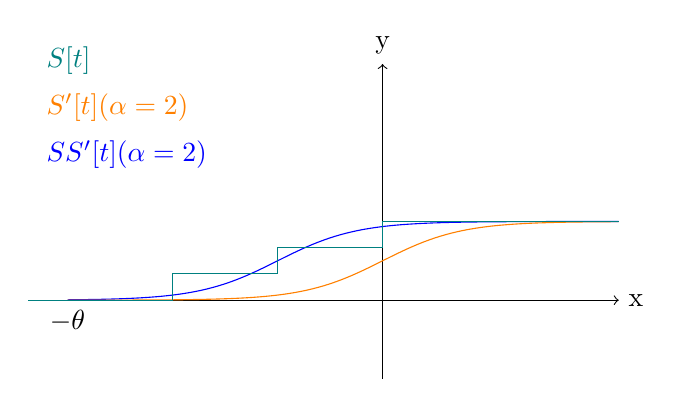
\begin{tikzpicture}
                \draw[->] (-4.5,0) -- (3,0) node[right] {x};
                \draw[->] (0,-1) -- (0,3) node[above] {y};
                \draw[color=blue] plot[domain=-4:3, samples=100] (\x, {1/(1 + exp(-2*(\x + 1/3*4)))});
                \draw[color=orange] plot[domain=-4:3, samples=100] (\x, {1/(1 + exp(-2*\x))});
                \draw[color=teal] (-4.5,0) -- (-4,0) node[below, color=black]{$-\theta$} -- (-2/3*4,0) -- (-2/3*4,1/3) -- (-1/3*4,1/3) -- (-1/3*4,2/3) -- (0,2/3) -- (0,1) -- (3,1);
                \matrix [draw=none, below left, anchor=north west] at (current bounding box.north west) {
                    \node [teal]{$S[t]$}; \\
                    \node [orange]{$S'[t](\alpha=2)$}; \\
                    \node [blue]{$SS'[t](\alpha=2)$}; \\
                };
            \end{tikzpicture}
            \caption{$n=2$}
        \end{subfigure}
        \hfill
        \begin{subfigure}[H]{\textwidth}
            \centering
            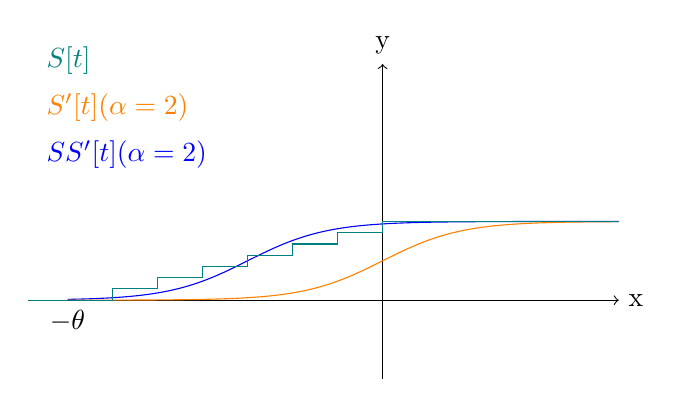
\begin{tikzpicture}
                \draw[->] (-4.5,0) -- (3,0) node[right] {x};
                \draw[->] (0,-1) -- (0,3) node[above] {y};
                \draw[color=blue] plot[domain=-4:3, samples=100] (\x, {1/(1 + exp(-2*(\x + 3/7*4)))});
                \draw[color=orange] plot[domain=-4:3, samples=100] (\x, {1/(1 + exp(-2*\x))});
                \draw[color=teal] (-4.5,0) -- (-4,0) node[below, color=black]{$-\theta$} -- (-6/7*4,0) -- (-6/7*4,1/7) -- (-5/7*4,1/7) -- (-5/7*4,2/7) -- (-4/7*4,2/7) -- (-4/7*4,3/7) -- (-3/7*4,3/7) -- (-3/7*4,4/7) -- (-2/7*4,4/7) -- (-2/7*4,5/7) -- (-1/7*4,5/7) -- (-1/7*4,6/7) -- (0,6/7) -- (0,1) -- (3,1);
                \matrix [draw=none, below left, anchor=north west] at (current bounding box.north west) {
                    \node [teal]{$S[t]$}; \\
                    \node [orange]{$S'[t](\alpha=2)$}; \\
                    \node [blue]{$SS'[t](\alpha=2)$}; \\
                };
            \end{tikzpicture}
            \caption{$n=3$}
        \end{subfigure}
        \caption{Comparison of Sigmoid Function, Shifted Sigmoid Function and Multi-bit Spike Train Model: $S[t]$ is the output spikes of the multi-bit spike train model, $S'[t]$ is the output spikes of the sigmoid function, $SS'[t]$ is the output spikes of the shifted sigmoid function}
        \label{fig:shifted_sigmoid}
    \end{figure}

\section{Implementation}
\label{sec:implementation}

    We use the SNN framework SpikingJelly which is based on PyTorch to implement the multi-bit spike train model. The firing mechanism is implemented as a forward path of the surrogate function in SpikingJelly. One just needs to override the Heaviside step function with the multi-bit spike train model. The core implementation is shown in Figure \ref{listing:multi-bit-spike}.
    \begin{figure}[!htpb]
        \centering
        \begin{lstlisting}[language=Python, basicstyle=\small, breaklines=true, numbers=left, stepnumber=1]
@torch.jit.script
def multi_level(x: torch.Tensor, n: int, threshold: float):
    l = int(2**n)-1
    r = (x >= 0).float()
    for i in range(1, l):
        r += ((x >= -float(i)/l * threshold) ^ (x >= -float(i-1)/l * threshold)) * float(l-i)/l
    return r.to(x)

class sigmoid(torch.autograd.Function):
    @staticmethod
    def forward(ctx, x, alpha, n, threshold):
        shift = (2**(n-1) -1) / (2**n-1) * threshold
        if x.requires_grad:
            ctx.save_for_backward(x+shift)
            ctx.alpha = alpha
            ctx.n = n
            ctx.threshold = threshold
        return multi_level(x, n, threshold)

    @staticmethod
    def backward(ctx, grad_output):
        return sigmoid_backward(grad_output, ctx.saved_tensors[0], ctx.alpha, ctx.n, ctx.threshold)

class Sigmoid(SurrogateFunctionBase):
    def __init__(self, alpha=4.0, spiking=True, n=1, threshold=1.0):
        super().__init__(alpha, spiking, n, threshold)

    @staticmethod
    def spiking_function(x, alpha, n, threshold):
        return sigmoid.apply(x, alpha, n, threshold)

    @staticmethod
    def backward(grad_output, x, alpha, n, threshold):
        shift = (2**(n-1) -1) / (2**n-1) * threshold
        return sigmoid_backward(grad_output, x+shift, alpha, n, threshold)[0]
        \end{lstlisting}
        \caption{Implementation of the Multi-bit Spike Train Model in SpikingJelly}
        \label{listing:multi-bit-spike}
    \end{figure}

    Noticing that the input $x$ is already centered to zero by SpikingJelly, so we apply the shift directly to the sigmoid function. 
